\documentclass[aip,jcp,reprint]{revtex4-2}

\usepackage{amsmath,amssymb,bm}
\usepackage{graphicx}
\usepackage{physics}
\usepackage{siunitx}
\usepackage{hyperref}

\begin{document}

\title{Application of the aperiodic defect model to a negatively charged vacancy in phosphorene}

 \author{Charlotte Rickert}
 \affiliation{Institut f\"ur Chemie, Humboldt-Universit\"at zu Berlin, Brook-Taylor-Str. 2, Berlin 12489, Germany}
 \affiliation{Max Planck Institute for Solid State Research, Heisenbergstr. 1, 70569 Stuttgart, Germany}

 \author{Lily Barta}
 \affiliation{Institut f\"ur Chemie, Humboldt-Universit\"at zu Berlin, Brook-Taylor-Str. 2, Berlin 12489, Germany}
 \affiliation{Max Planck Institute for Solid State Research, Heisenbergstr. 1, 70569 Stuttgart, Germany}

 
 \author{Ernst-Christian Flach}
 \affiliation{Institut f\"ur Chemie, Humboldt-Universit\"at zu Berlin, Brook-Taylor-Str. 2, Berlin 12489, Germany}

 
\author{Daniel Kats}%
\affiliation{Max Planck Institute for Solid State Research, Heisenbergstr. 1, 70569 Stuttgart, Germany}%

 
 \author{Denis Usvyat}
 \affiliation{Institut f\"ur Chemie, Humboldt-Universit\"at zu Berlin, Brook-Taylor-Str. 2, Berlin 12489, Germany}
 \email{denis.usvyat@hu-berlin.de}

 

\date{\today}

\begin{abstract}
  Point defects critically influence the structural and electronic properties of two-dimensional materials.
  %In phosphorene, single vacancies reconstruct into a 5–9 defect geometry that introduces localized in-gap states. Traditional density functional theory (DFT) provides structural insight, but accurate treatment of correlation—especially for charged defect states—remains challenging.

%Here, we investigate neutral and negatively charged vacancies in phosphorene using an aperiodic defect model: an HF-embedded cluster for the environment and a correlated coupled cluster treatment of the defect-centered fragment. Optimized 5–9 geometries are obtained from periodic B3LYP-D3 calculations on a $3\times4$ supercell using the pob-TZVP-rev2 basis set within \textsc{CRYSTAL}. Energetics, defect levels, and charge localization are analyzed, highlighting the importance of high-level correlated descriptions tailored to defect physics.
\end{abstract}

\maketitle


\section{Introduction}

Elemental phosphorus is an intriguing material for chemical and technological applications, particularly due to the diversity of its allotropes and their properties. Under standard conditions, the semiconducting black phosphorus allotrope has traditionally been considered the most thermodynamically stable form of phosphorus\cite{Keyes1953,Cartz1979} (although recent studies suggest that violet phosphorus may be slightly more stable within methodological uncertainty.\cite{Bonometti2025,Vogt2023}).  Black phosphorus consists of a three-dimensional stacking of  covalent monolayers bound by weak van der Waals interactions.\cite{Morita1986,our_calculation,luke} An individual monolayer, referred to as phosphorene, is of considerable interest in its own right as a two-dimensional material with strong potential for applications in single-layer electronics,\cite{Li2014BPTransistor,Liu2014PhosphoreneTransistor,Zhang2024} optoelectronics,\cite{Xia2014RediscoveringBP,Zhang2024} catalysis, and other application domains.\cite{CastellanosGomez2015Review,Tian2023}

As in many low-dimensional materials, the properties of phosphorene can be strongly affected by the presence of point defects such as vacancies or substitutional impurities. Generally, in semiconductors, such defects may reduce charge carrier mobility by acting as scattering or trapping centers.\cite{Shockley1952,Hall1952,Stoneham2001} At the same time, the controlled incorporation of impurity atoms is essential for semiconductor technology, as shallow donor and acceptor states enable control of carrier concentrations.\cite{Sze2006,YuCardona2010} Beyond electronic transport, point defects can also modify chemical reactivity and catalytic activity by creating localized active sites.\cite{Freund2011} In addition, certain defects host localized electronic states of interest for quantum technologies.\cite{Doherty2013,Awschalom2018}

Point defects in phosphorene, in particular the vacancies, have therefore attracted considerable theoretical attention.\cite{Hu2015VacancyBP,Ziletti2015,Carvalho2016Review,Kundu2020NativeDefectsPhosphorene,Srivastava2015VacanciesPhosphorene,Speckmann2024ElectronBeamDefects,ElKhatib2024PhosphoreneMoS2Vacancies,Huang2023VacancyPNR} Previous studies have shown that the monovacancy undergoes a substantial local reconstruction accompanied by rebonding of neighboring atoms\cite{Hu2015MonoDiVacancies,Wang2015NativeDefects} and introduces localized electronic states within the band gap.\cite{Guo2015VacancyStates,Srivastava2015VacanciesAdatoms} The monovacancies in phosphorene have been predicted to act as acceptor-like defects and may contribute to the commonly observed p-type character of black phosphorus.\cite{Wang2015NativeDefects} In addition, the migration barrier of the vacancy is relatively low, suggesting that such defects may be highly mobile and dynamically active under suitable conditions.\cite{Cai2016VacancyMobility}


Most computational investigations of point defects in general employ density functional theory (DFT) within the periodic supercell approach (i.e. periodic defect model), where the defect placed in a large cell is periodically repeated.\cite{Freysoldt2014Review} While this approach has proven successful, it inherently introduces artificial periodicty causing non-physical interactions between the defect and its replicas, and other issues. These finite-size effects may compromize the description of isolated defects and slow down convergence to the thermodynamic limit. Particularly problematic are charged defects, whose periodization requires an unphyscal compensating background and associated finite-size corrections.\cite{Freysoldt2009ChargeCorrection,Lany2008FiniteSizeErrors} Another challenge is description of defects beyond DFT. Wavefunction-based methods, such as for example coupled cluster theory, provide systematic hierarchies of progressively more accuraty description, but for large supercells they are computationally prohibitive. A promising route is offered by embedding strategies that restrict the computatioanllly expensive high-level correlated treatment to the defect region while the environment is represented by a lower-level description.\cite{Sun2016EmbeddingReview,..}


In this work we apply the recently developed aperiodic defect model (ADM)\cite{...} to study a negatively charged vacancy in a phosphorene monolayer. In contrast to the supercell model, ADM describes a single defect embedded in an otherwise non-defective crystal and thus avoids the artificial periodicity of the supercell calculations and lifts the necessity for the compensating background charge.  In the absence of the parasitic long-range defect–defect interactions the convergence toward the thermodynamic limit in ADM is expected to be faster. Furthermore, since ADM reduces the problem to an effective molecular-like calculation, it enables the straightforward application of highly accurate molecular quantum-chemical methodologies for the description of both ground and excited states.

Nevertheless, phosphorene represents a challenging test case for the ADM. The material forms a covalently bonded network that can undergo substantial structural rearrangement in the presence of a vacancy. In combination with the relatively high polarizability of phosphorene, this may lead to a long-range response to the defect and consequently to a slow convergence with respect to fragment size. In addition, the relatively narrow band gap may cause poorer orbital localization, which can obscure a fragment-based partitioning. Finally, the present work considers ground and excited states of a charged defect, whose spatial locality and thus rapid convergence with fragment size is not guaranteed. For these reasons, the negatively charged vacancy in phosphorene provides a demanding test case for assessing the capabilities of the ADM.


%Two-dimensional (2D) phosphorene has attracted intense interest due to its semiconducting direct band gap and high carrier mobility. However, intrinsic defects such as single vacancies significantly alter its properties, acting as scattering centers, charge traps, or dopants. Vacancies are also implicated in enhanced chemical reactivity and degradation mechanisms, such as oxidation and humidity-driven deterioration.

%**Previous computational studies** have comprehensively characterized point defects in phosphorene. Early first-principles investigations revealed a variety of vacancy and reconstructed configurations with relatively low formation energies compared to other 2D materials, such as graphene or silicene \cite{HuYang2015_JPCCdefects}. The single vacancy commonly relaxes into a reconstructed 5–9 structure introducing mid-gap states, sometimes magnetic or acceptor-like in nature \cite{HuYang2015_JPCCdefects, PhysRevB.91.045433}. Density functional theory (DFT) combined with many-body GW corrections has further shown that vacancy defects have low formation energies (0.9–1.6\,eV) and can explain p-type conductivity in phosphorene \cite{PhysRevMaterials.4.054004}. Charged vacancy states were predicted to be stable in $-1$ charge configurations, significantly modifying local geometry and reactivity \cite{Zhan2019_JPCCvacancies}. DFT-based molecular dynamics and neural-network potentials have also studied vacancy mobility, showing that monovacancies are highly itinerant—especially along the zigzag direction—leading to coalescence into energetically favorable divacancies \cite{JPhysChemC.3c05713}.

%**Experimental observations** of monovacancies remain challenging due to rapid diffusion and coalescence, although advanced microscopy has begun to resolve individual vacancy clusters. Vacancies also correlate with mechanical degradation; for example, molecular dynamics studies indicate that even low vacancy concentrations substantially degrade fracture strength \cite{Sha2016_Nanotechnology}. Vacancy sites preferentially serve as adsorption and reaction centers for atmospheric species such as O$_2$, consistent with rapid phosphorene degradation seen experimentally \cite{Kistanov2016_arXivoxidation}.

%Despite the wealth of DFT-based studies, the accurate description of charged defect states and associated correlation effects beyond semi-local or hybrid functionals remains an open challenge. Standard periodic approaches also suffer from finite-size charge correction issues.



%Here, we combine a periodic DFT-optimized 5–9 reconstructed geometry with an aperiodic HF-embedded defect cluster treated at the coupled cluster level to accurately describe neutral and negatively charged vacancies in phosphorene.

\section{Theory: Aperiodic Defect Model}


The details of the aperiodic defect model can be found in Ref.~\onlinecite{Lavroff2025_JCP_ADM}; here we provide only a conceptual overview. In ADM the first step is a periodic restricted Hartree--Fock (HF) calculation on a non-defective host crystal. The localized occupied orbitals --- Wannier functions (WFs) --- from this calculation\cite{Zicovich_Dovesi_WFs} are then used to partition the system into the environment and the fragment. The environment remains frozen in the periodic HF solution, while the fragment geometry is subsequently manipulated to create the defect and its electronic structure is recalculated.

The fragment containing the defect is then subjected to an effectively molecular-like calculation, with the embedding field from the frozen environment implicitly included in the fragment's one-electron Hamiltonian $h^{\rm def}$ through the Fock matrix $F^{\rm per}$ from the non-defective periodic HF calculation:
\begin{eqnarray}
h^{\rm def}_{\mu'\nu'}&=&F^{\rm per}_{\mu'\nu'}-\sum_{i\in{\rm frag}}\left[2\left(\mu'\nu'|ii\right)
  - \left(\mu' i|i \nu'\right)\right]\\
&-& \bra{\mu'} \sum_{K'\in{\rm add}}{Z_{K'} \over |{\bf r}-{\bf
    R}_{K'}|}-\sum_{K\in{\rm rem}}{Z_{K} \over |{\bf r}-{\bf
                          R}_{K}|}\ket{\nu'}.\label{eq:defect_h}
\end{eqnarray}
Here $(\mu'\nu'|ii)$ and $(\mu' i|i \nu')$ are the Coulomb and exchange integrals in the usual chemical notation, with $i\in{\rm frag}$ being the fragment-defining occupied WFs from the pristine HF calculation. The summations in eq.~(\ref{eq:defect_h}) over $K$ and $K'$ are carried out only over the manipulated atoms, i.e., the removed ones $(K)$ and the added ones $(K')$.


The AO-like basis orbitals $\ket{\mu'}$ are obtained by projecting the atomic orbitals (AOs) of the fragment atoms (after defect formation) from the occupied WFs of the environment $i\notin{\rm frag}$:
\begin{eqnarray}
  \left|\mu'\right>=(1-\sum_{i\notin{\rm frag}}\left|i\right>\left<i\right|
  )\left|\mu\right>.\label{eq:new_AO}
\end{eqnarray}
This projection guarantees orthogonality of the fragment orbital space to the occupied manifold of the frozen environment and at the same time allows the use of atom-centered basis functions with the same nomenclature as the usual AOs. The fragment atoms that serve as centers for the basis orbitals (as well as auxiliary functions for density fitting) are chosen using the orbital-domain machinery of local correlation methods.\cite{Usvyat_periodic_LMP2} The atomic fragment is thus defined as the union of the centers that enter the domains of the fragment-defining WFs.
In practice, since atomic fragments are easier to control and visualize, the fragment is specified in terms of atoms. The actual orbital fragment is then defined by the WFs whose domains are fully contained within the atomic fragment. By default, the standard Boughton--Pulay domains\cite{Boughton1993} with a tolerance of 0.98 are used, which typically leads to one-atom domains for lone-pair WFs and two-atom domains for bonding WFs. The domains, and thus the set of AO centers for the fragment, can also be extended using, for example, distance-based or bond-connectivity criteria.


The number of electrons in the fragment is determined by the fragment WFs rather than by the formal charge of the fragment atoms:
\begin{eqnarray}
  N_{\rm el}^{\rm frag}=2N_{\rm WFs}^{\rm frag}-\sum_{K\in{\rm rem}}Z_{K}+\sum_{K'\in{\rm add}}Z_{K'}+\Delta_{\rm el},\label{eq:n_el}
\end{eqnarray}
where $N_{\rm WFs}^{\rm frag}$ is the number of initial WFs that define the fragment, $Z_{K}$ and $Z_{K'}$ are the nuclear charges of the removed and added atoms of the defect, respectively, and $\Delta_{\rm el}$ is the number of added or removed electrons if the defect is charged. A possible excess in the nuclear charge in the fragment is conceptually unproblematic, as it is compensated by the environment electrons. It therefore only adds a constant energy component to the total energy, which cancels in energy differences.






The energy of the system is defined as the energy of the finite fragment subjected to the periodic embedding field. This leads to standard expressions for the HF or correlation energy formally equivalent to those of an isolated finite cluster in an AO basis, but with modified Hamiltonian matrix elements and an effective nuclear energy $E^{\rm def}_{\rm nuc}$. The one-electron Hamiltonian in Eq.~(\ref{eq:defect_h}) contains additional terms compared to the standard one-electron Hamiltonian, while the two-electron part is represented by the standard electron repulsion integrals. In addition, both one- and two-electron parts involve the projected fragment AOs $\ket{\mu'}$, which are linear combinations of AOs from both the fragment and the environment, see Eq.~(\ref{eq:new_AO}). Finally, the nuclear energy term also contains the contribution from the environment:
\begin{eqnarray}
  E^{\rm def}_{\rm nuc}&=&{1 \over 2}\sum_{K'\in{\rm add}}\sum_{L'\in{\rm add}}\phantom{}^{'}{Z_{K'}Z_{L'} \over |{\bf R}_{K'}-{\bf
      R}_{L'}|}\nonumber\\
  &&+\sum_{K'\in{\rm add}}\left[ Z_{K'}\cdot V\left({\bf
                          R}_{K'}\right) -\sum_{K\in{\rm rem}}\phantom{}^{'}{Z_{K}Z_{K'} \over |{\bf R}_{K}-{\bf R}_{K'}|}\right]\nonumber\\
  &&-2\sum_{i\in{\rm frag}}\left< i\left|-\sum_{K'\in{\rm add}}{Z_{K'} \over |{\bf r}-{\bf  R}_{K'}|}\right|i\right>,\label{eq:E_nuc_defect}
  \end{eqnarray}
where $V\left({\bf R}_{K'}\right)$ is the elctrostatic potential from the periodic host crystal at the position of the added atoms. 
Again the summations over nuclei run only over the removed or added ones rather than over all nuclei of the fragment. This restriction only affects a constant energy shift which cancels out in energy differences.\cite{Lavroff2025_JCP_ADM}

The density-fitted ADM has been implemented in the \textsc{Cryscor} program\cite{CRYSCOR} by repurposing the local density-fitting machinery of the periodic LMP2-F12 code.\cite{Usvyat2013_F12} Density-fitted Hartree--Fock and canonical MP2 calculations are carried out on the \textsc{Cryscor} side. Higher-level methods are run via an interface to the molecular code \textsc{Molpro},\cite{Molpro2020} which is straightforward due to the formal equivalence between ADM and a finite cluster. 

In this work we employ the canonical four-index integral \texttt{FCIDUMP} interface,\cite{Knowles1989_FCIDUMP} which is used for DCSD,\cite{..} CCSD(T),\cite{..} and EOM-CCSD\cite{..} calculations. In addition, we test an interface to our pilot implementation of density-fitted local correlation methods,\cite{your_local_corr_ref} currently featuring local MP2, local DCSD, and local ADC(2)\cite{..}. These methods employ Pipek--Mezey localization\cite{Pipek1989} of the fragment HF orbitals together with the PAO-domain restricted virtual space and are implemented within the local integrated tensor framework\cite{Kats_LITF} of the \textsc{Molpro} program package.



\section{Computational parameters}


Unless specified otherwise, all calculations employed the POB-VTZ-rev2 basis set.\cite{POB_VTZ-rev2} Periodic DFT and HF calculations were performed with the \textsc{CRYSTAL17} program.\cite{CRYSTAL} Structural optimizations were carried out using the B3LYP functional\cite{B3LYP1} with the D3 dispersion correction.\cite{GrimmeD3}
SCF convergence was stabilized by damping the Fock matrix updates to 20\% during the initial iterations. The DIIS acceleration procedure was activated only after the energy change dropped below $0.01$~hartree.

The structure of pristine phosphorene was obtained using a $12\times12$ $k$-mesh and a slightly modified POB-VTZ basis set, where the $d$- and $f$-type functions were taken from the cc-pVTZ basis.\cite{Dunning1989}
The defect structure was optimized in a $4\times3$ supercell (48 atoms) with one excess electron per cell to model the negatively charged vacancy and using a $12\times12$ $k$-mesh. To allow a possible spin-polarization on the defect, it was  treated using broken-symmetry DFT with an initial triplet guess.


In the periodic HF calculations within ADM, the integral tolerances were tightened significantly relative to the default values to minimize numerical errors in the embedding field. Specifically, the  \textsc{CRYSTAL} TOLINTEG thresholds were set to 10 10 10 30 100, and a $16\times16$ $k$-mesh was employed. Formally, the periodic HF calculation for ADM could be performed in the primitive unit cell. In practice, however, \textsc{CRYSTAL} cannot evaluate the periodic Fock matrix $F^{\rm per}_{\mu'\nu'}$ for basis functions centered on displaced atoms when they appear too close to each other, which turned out to be the case within the primitive cell set up. Therefore, a $2\times2$ supercell was employed for the periodic HF step.

In the present density-fitted implementation of ADM, the same auxiliary fitting basis is employed for both HF and post-HF two-electron integrals. Consequently, the auxiliary basis must provide adequate accuracy for both contributions. Test calculations show that the HF energy is considerably more sensitive to the choice of the auxiliary basis than the correlation energy, a behavior that has also been observed in other studies.\cite{DF_HF_sensitive}
Therefore, our auxiliary basis is based on the cc-pVTZ/JKFIT set,\cite{Weigend2002_JKFIT} which was optimized specifically for HF calculations. In this basis, the $f$- and $g$-type functions were replaced by those from the cc-pVTZ/MP2FIT auxiliary basis,\cite{Weigend2002_MP2FIT} which contains a richer set of high-angular-momentum functions. Such a combination has been found to provide high accuracy in energy differences for both the HF and correlation contributions calculated with POB-VTZ-rev2.


The fragment HF and MP2 calculations within ADM were carried out using our ADM implementation in the \textsc{Cryscor} code. Other fragment post-HF calculations were performed with \textsc{Molpro} via the \texttt{FCIDUMP} interface\cite{Knowles1989_FCIDUMP} (DCSD, CCSD(T), EOM-CCSD) or through our own interface to the local integrated tensor framework (LITF)\cite{Kats_LITF} (LMP2, LDCSD, CIS, LADC(2)). 

The current LDCSD implementation within LITF is restricted to strong pairs, defined as pairs that share at least one atom in their respective orbital domains. The remaining pairs, denoted as weak pairs, are treated at the LMP2 level. For the ground-state amplitudes, the standard orbital domains extended by one bond connectiveity (iext=1) were used.

Reference calculations for the phosphorus atom in its quartet ground state were also carried out using \textsc{Molpro} with ROHF,\cite{Roothaan1960_ROHF} RMP2,\cite{Pople1976_RMP2} RDCSD,\cite{RDCSD_ref} and RCCSD(T).\cite{RCCSDT} To reduce basis-set superposition error, the phosphorus atom was surrounded by 11 ghost centers placed at the positions of neighboring atoms in the pristine phosphorene structure (for local methods it was 3 ghost atoms to mimic the iext=1 domains). All post-HF methods use the frozen core approximation.


Finally, the periodic CIS optical band gap of pristine phosphorene was computed using the \textsc{Cryscor} CIS implementation described in Ref.~\onlinecite{Cryscor_CIS}.



\section{Structural specification of ADM}

A B3LYP-D3 optimization of pristine phosphorene (Fig.~\ref{fig:per_phos}a) yields lattice parameters of $a=3.30\,\text{\AA}$ and $b=4.47\,\text{\AA}$ (the full structural specification is provided in the Supporting Information). Two reconstructed monovacancy structures are typically considered in phosphorene: the asymmetric (5|9) and the symmetric (55|66) configurations, denoted according to the number of atoms forming the rings. To compare these configurations energetically, we optimized the defect in a $4\times3$ supercell starting from both symmetric and distorted initial geometries. To probe the spin symmetry of the wavefunction of the negatively charged monovacancy, we considered both triplet and singlet spin states. To prevent artificial trapping in a closed-shell solution in the singlet calculations, the initial guess orbitals were taken from preliminary triplet SCF runs allowing for possible spin polarization.


\begin{figure}
\centering
%\begin{tabular}{cc}
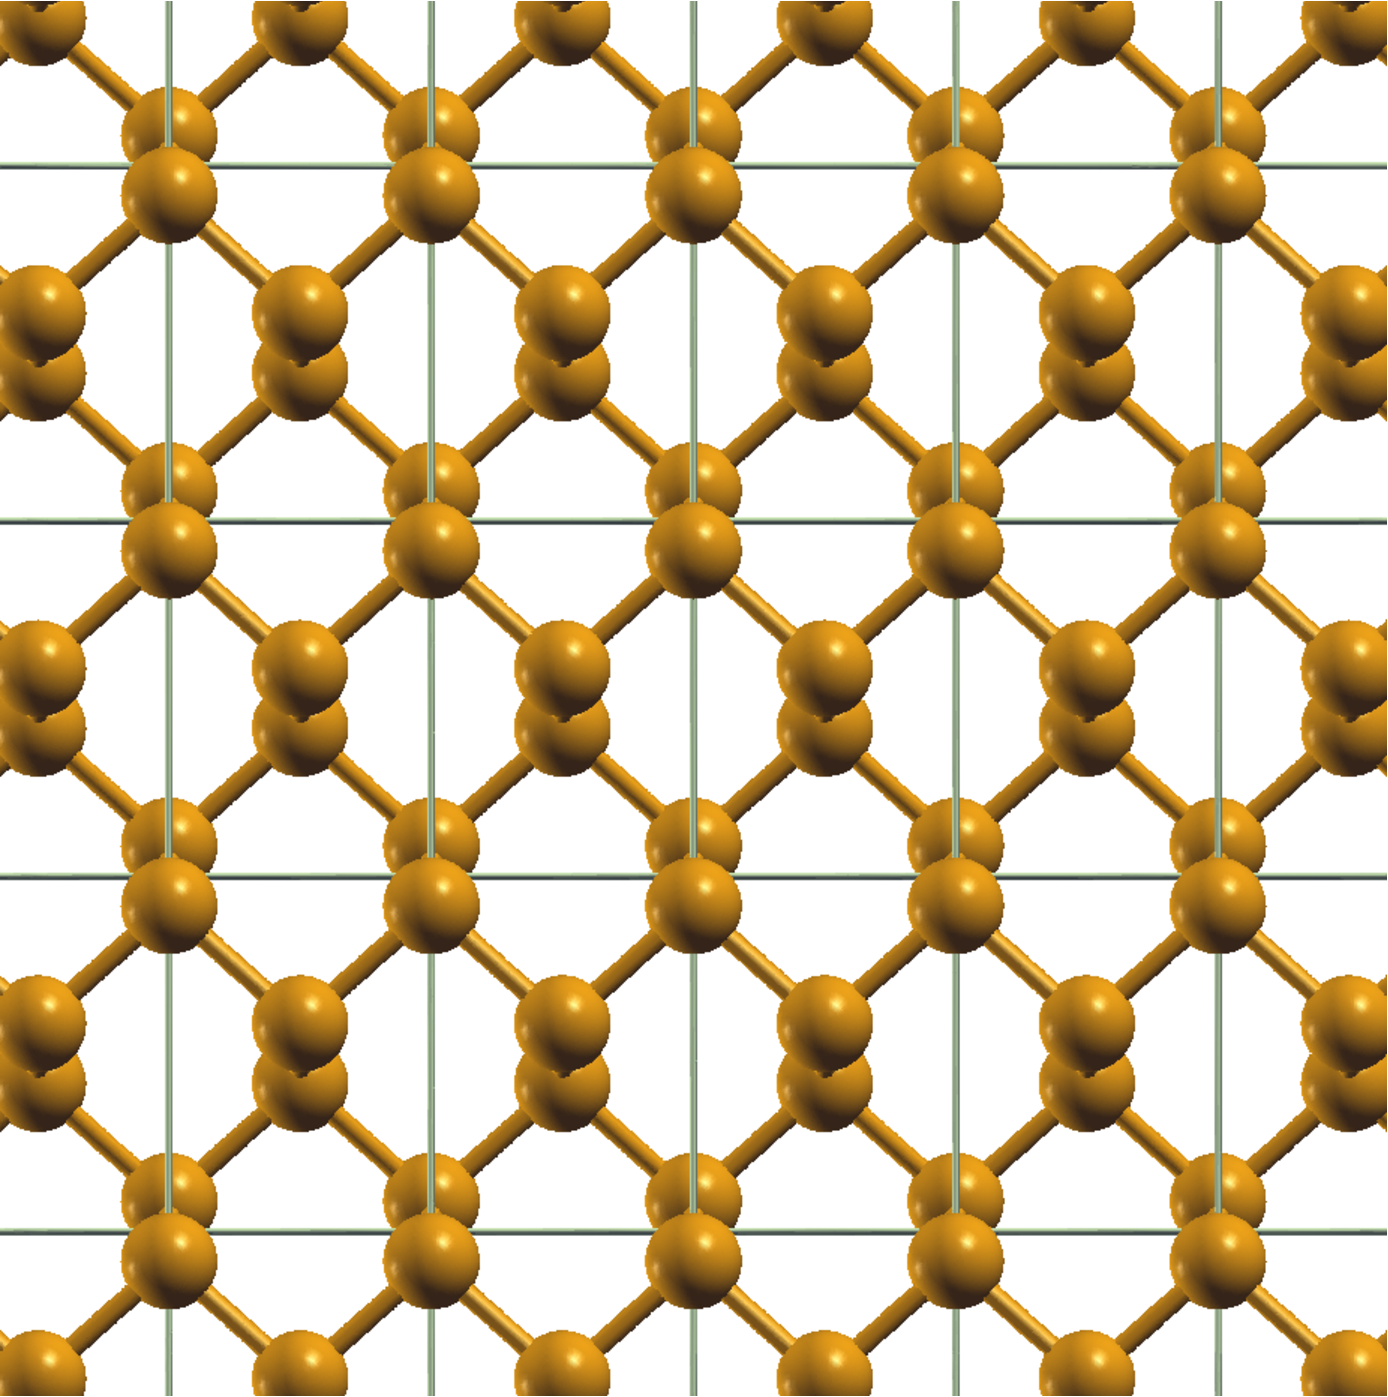
\includegraphics[width=0.45\textwidth]{Pristine.pdf}\\
(a)\\
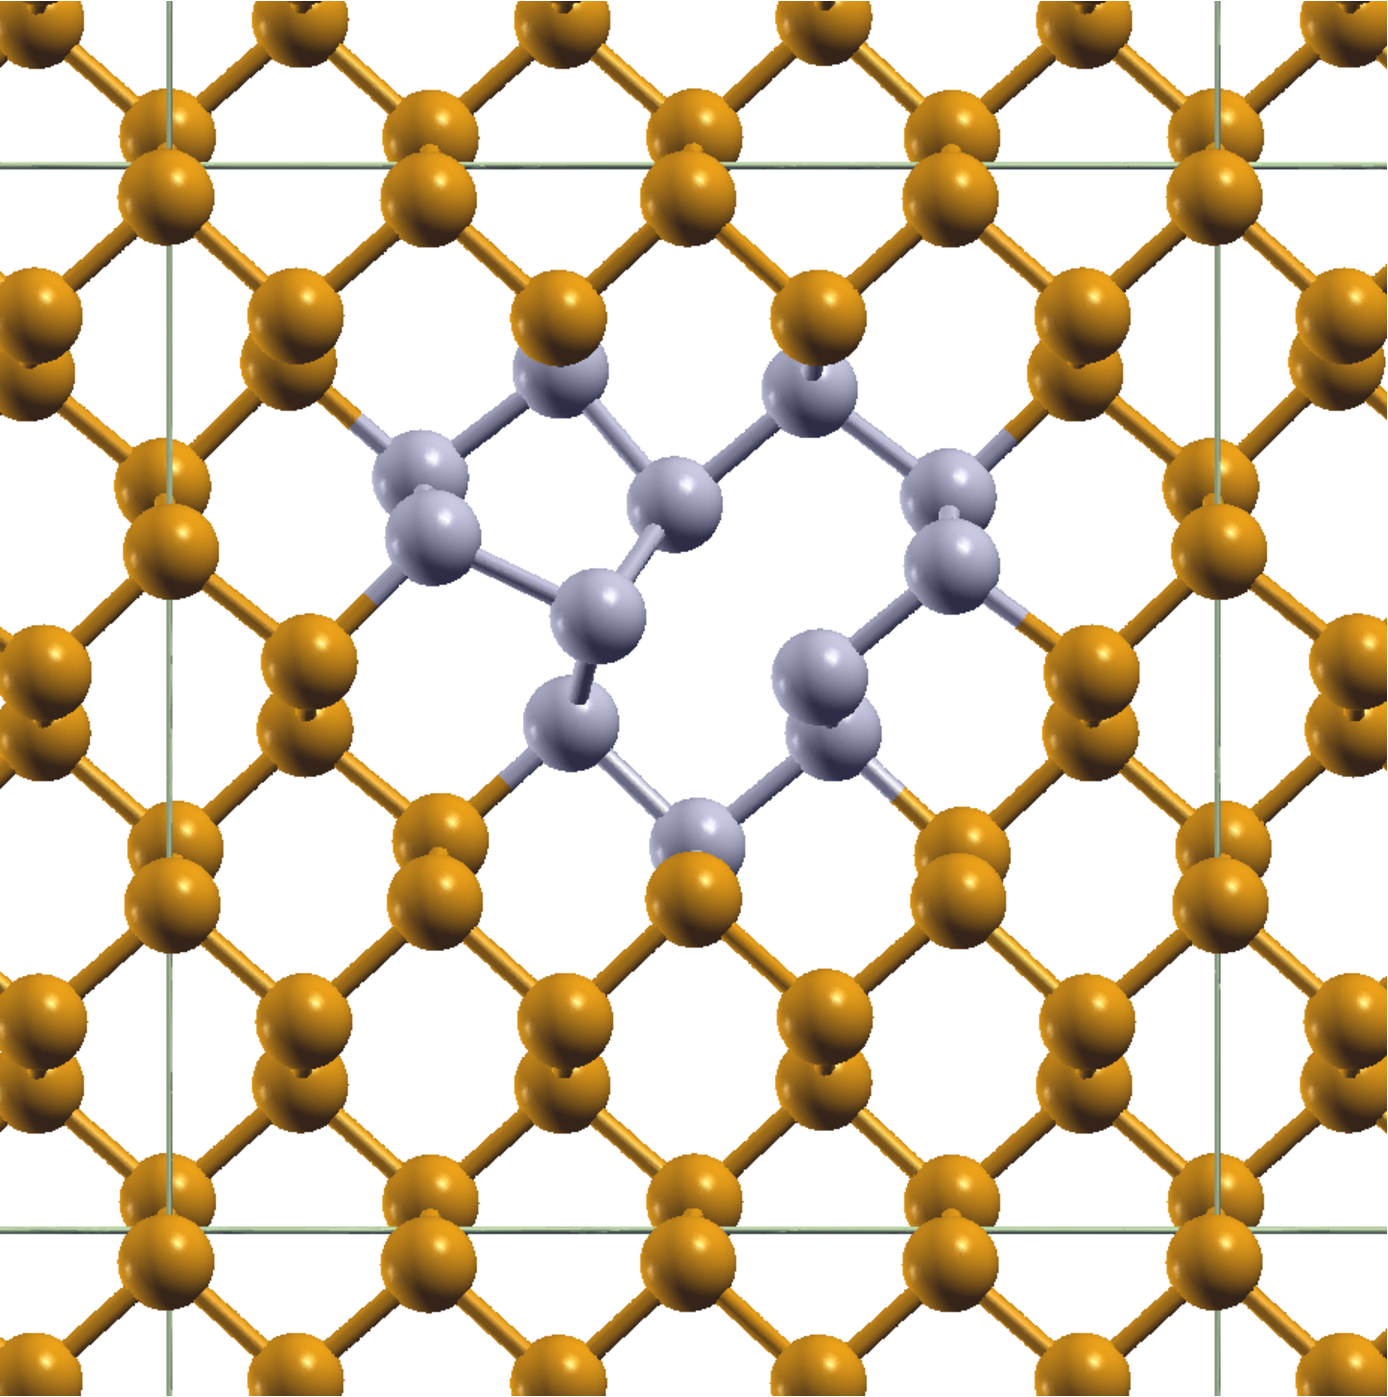
\includegraphics[width=0.45\textwidth]{Defect.pdf}\\
(b)
%\end{tabular}
\caption{Optimized structures of pristine phosphorene (a) and the negatively charged monovacancy in phosphorene within a $4\times3$ supercell (b). The structures of the pristine phoshphorene (a) and of the negatively charged (5|9)-vacancy in phosphorne optimized within 4$\times$3-supercell.  The atoms belonging to the reconstructed 5- and 9-membered rings are highlighted in grey.}\label{fig:per_phos}
\end{figure}


The optimized defect in the triplet state was found to be about 0.6 eV higher in energy than in the singlet state. When optimized starting from a distorted geometry, the singlet state converged to the (5|9) structure shown in Fig.~\ref{fig:per_phos}b. Furthermore, despite the spin-polarized initial guess,  at the (5|9) optimized geometry the wavefunction converged to a closed-shell solution.
Optimization starting from the symmetric structure resulted in a spin-polarized solution within the (55|66) geometry. However, this structure was slightly higher in energy (by about 0.34 eV), suggesting that it corresponds to a shallow transition state between the (5|9) and (9|5) minima. These results are consistent with previous DFT studies of 
phosphorene monovacancies.\cite{Hu2015_PhosphoreneVacancies,Naik2020_PRMaterials_PhosphoreneDefects,Rijal2021_PhosphoreneVacancy}




Following these results, we focus on the minimum (5|9) structure for the subsequent ADM calculations. To enable the ADM calculations on fragments smaller than the full 48-atom supercell -- necessary for computationally demanding post-Hartree–Fock methods -- the system was reoptimized within the same $4\times3$ supercell while allowing only a subset of atoms to relax. Restricting relaxation to the 12 atoms that form the 5- and 9-membered rings leads to a collapse toward the (55|66) structure, indicating that the relaxed fragment must be further expanded. Including all atoms that move by at least 0.1~\AA\ adds six additional atoms, yielding an 18-atom fragment that correctly relaxes to the (5|9) configuration. This set of 18 atoms thus defines the minimal fragment used in the subsequent ADM calculations, as the latter must encompass all displaced centers (see Fig.~\ref{fig:frags}). 


To assess the convergence with respect to fragment size, we consider a series of fragments containing up to 141 atoms. Each successive fragment is constructed by adding atoms within one bond connectivity from the previous fragment. The set of displaced atoms is kept fixed to the initially chosen 18 atoms (see Fig.~\ref{fig:frags}).


For the defect formation energy we employ its chemical definition as the electronic energy contribution to the energy of the model reaction
\[
\text{pristine phosphorene} \rightarrow \text{phosphorene with a vacancy} + \text{P atom}.
\]
Accordingly, the formation energy is given as
\begin{eqnarray}
  E_{\rm form}&=&\Delta E^{\rm ADM}({\rm HF}) + \Delta E^{\rm ADM}({\rm corr})\nonumber\\
  &&+\Delta E_{\rm 18\uparrow relax},\label{eq:energy}
\end{eqnarray}
where $\Delta E^{\rm ADM}$ is the formation energy within the ADM model,
\begin{eqnarray}
  \Delta E^{\rm ADM}=E^{\rm ADM}_{\rm defect} + E_P - E^{\rm ADM}_{\rm pristine}.
\end{eqnarray}
Here $E_P$ is the energy of the phosphorus atom in its quartet ground state, and $\Delta E_{\rm 18\uparrow relax}$ denotes the relaxation energy beyond the 18-atom fragment,
\begin{eqnarray}
  \Delta E_{\rm 18\uparrow relax}=E_{\rm relax} - E_{\rm relax\,18},
\end{eqnarray}
where $E_{\rm relax}$ is the energy of the fully relaxed structure and $E_{\rm relax\,18}$ is that of the structure with only the 18 atoms relaxed. With our $4\times3$ supercell and the B3LYP-D3 functional, $\Delta E_{\rm 18\uparrow relax}$ amounts to $-0.146$ eV.

We note that the definition (\ref{eq:energy}) corresponds to the reaction-energy formulation commonly used in quantum chemistry. It is equivalent to the standard solid-state expression for the defect formation energy\cite{Freysoldt2014Review}, provided that the phosphorus chemical potential is chosen as the energy of an isolated phosphorus atom. In contrast to periodic supercell approaches, charge and finite-size corrections are not required in ADM, as the latter does not involve periodic replication of the defect or the introduction of a compensating background charge. Instead, the charged defect explicitly experiences the electrostatic potential of the non-defective crystal through the embedding.



\begin{figure*}
\centering
\begin{tabular}{ccc}
  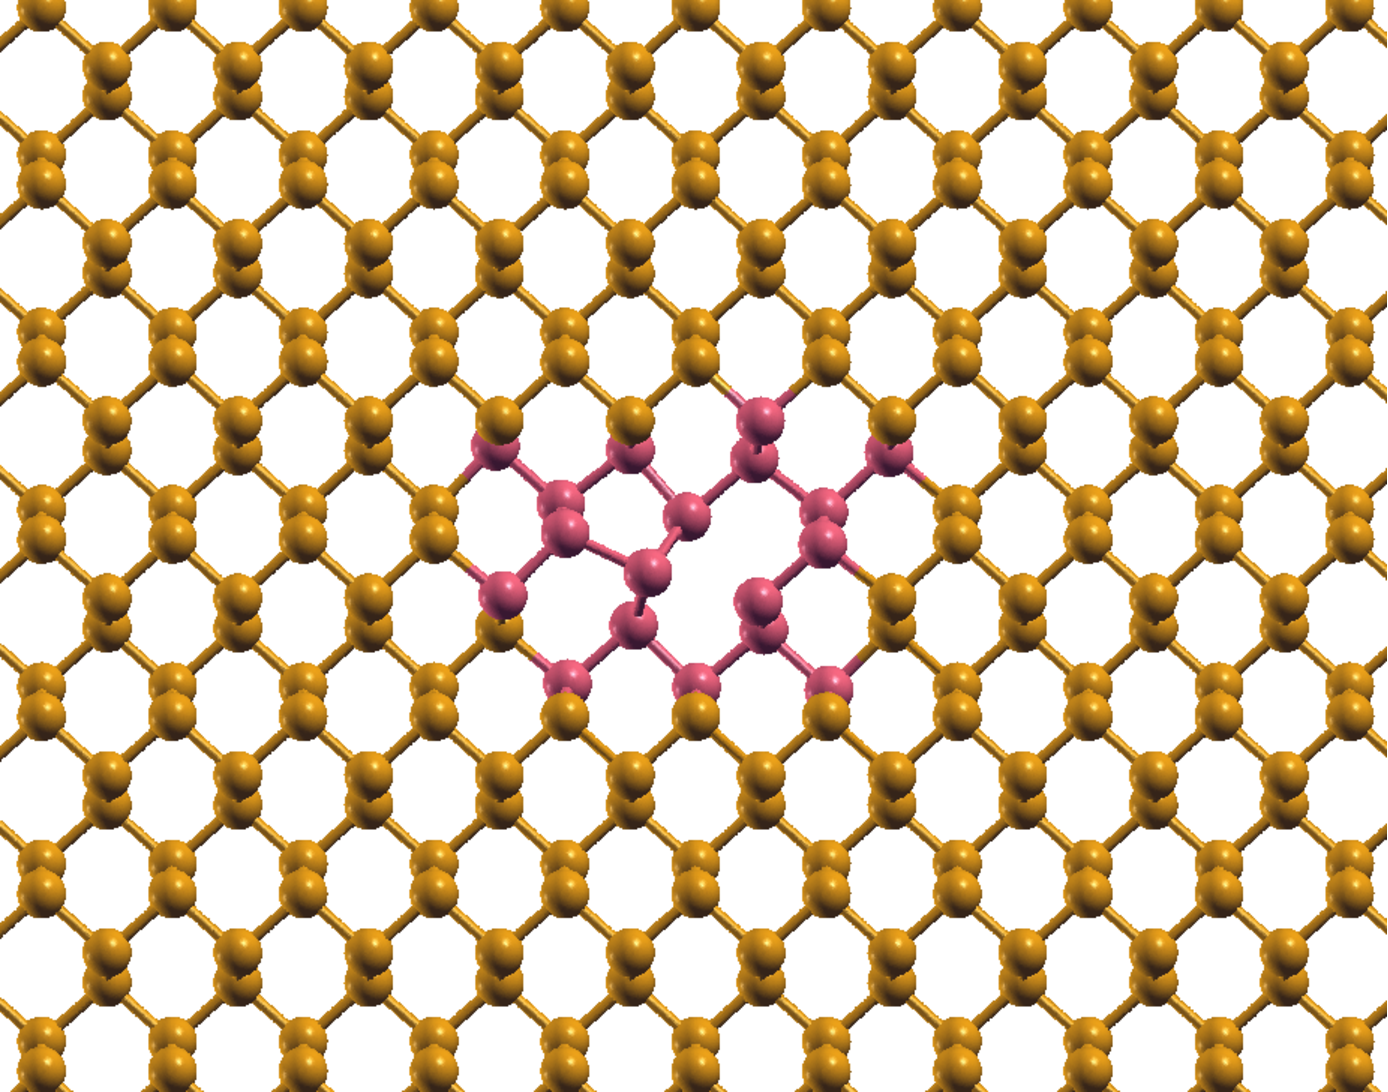
\includegraphics[width=0.3\textwidth]{18.pdf}&
  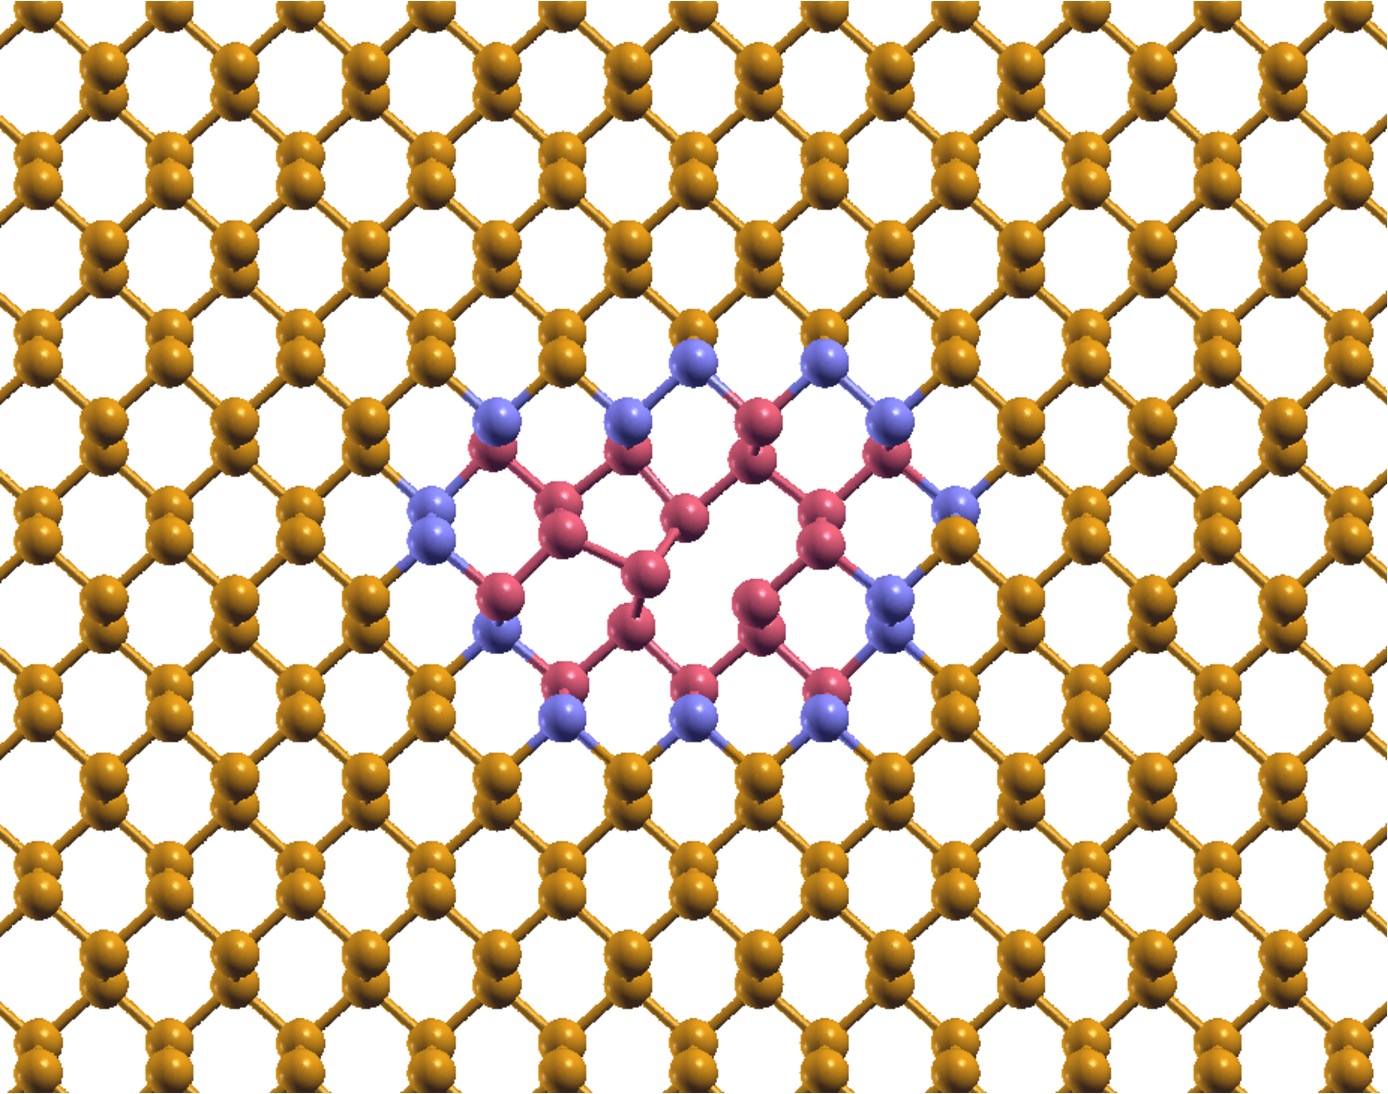
\includegraphics[width=0.3\textwidth]{32.pdf}&
  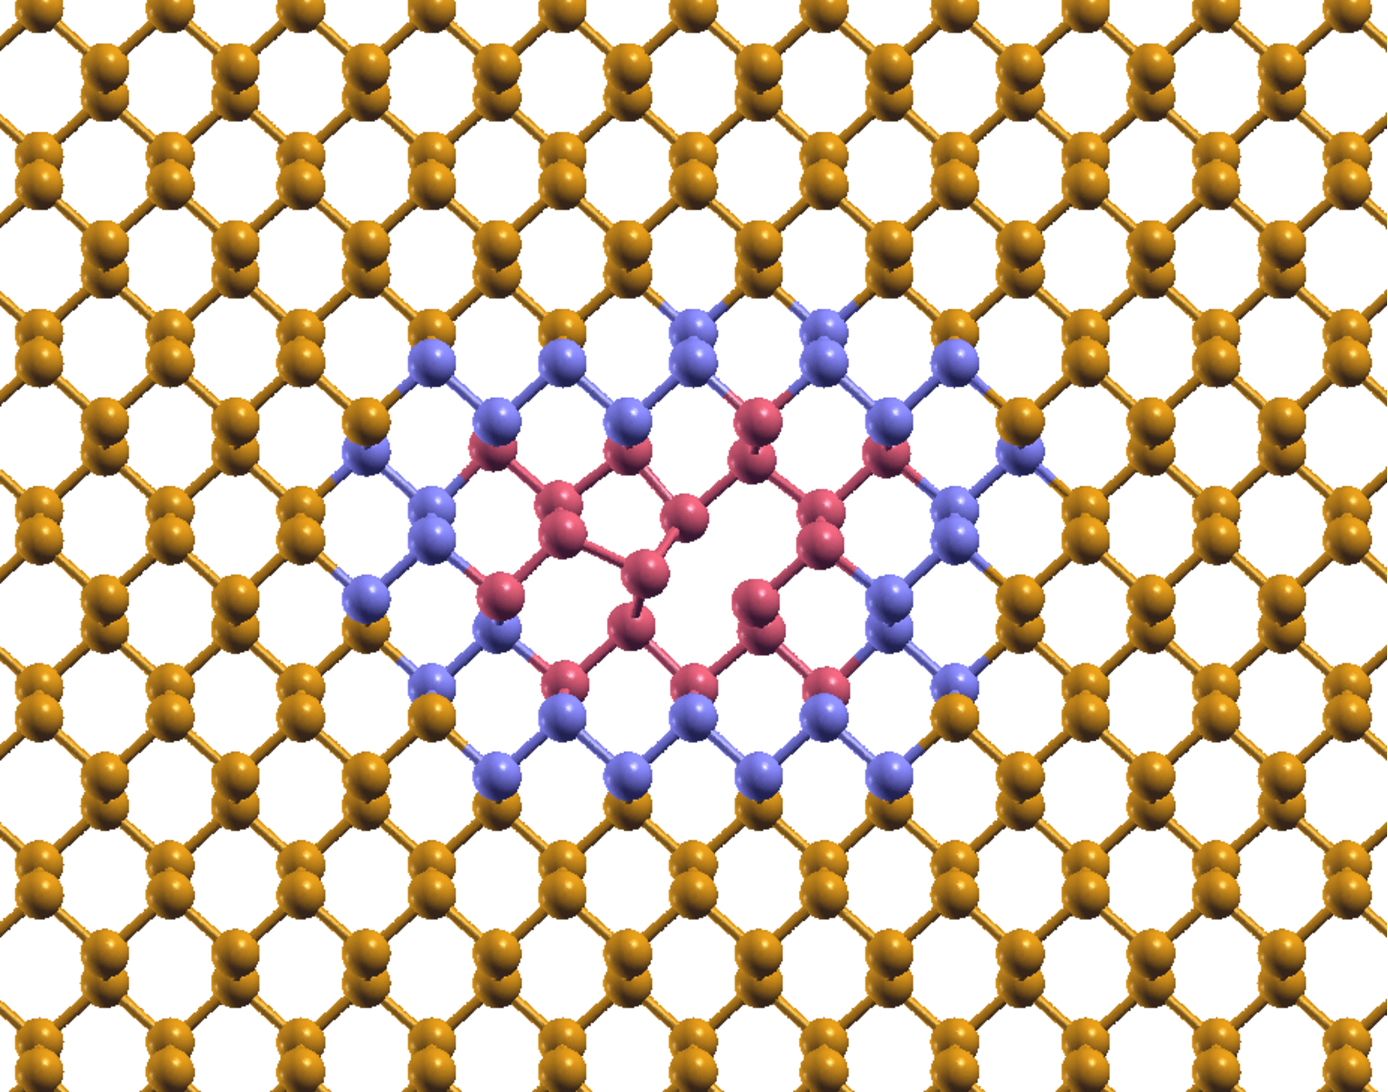
\includegraphics[width=0.3\textwidth]{47.pdf}\\
  18 atoms & 32 atoms & 47 atoms\\
  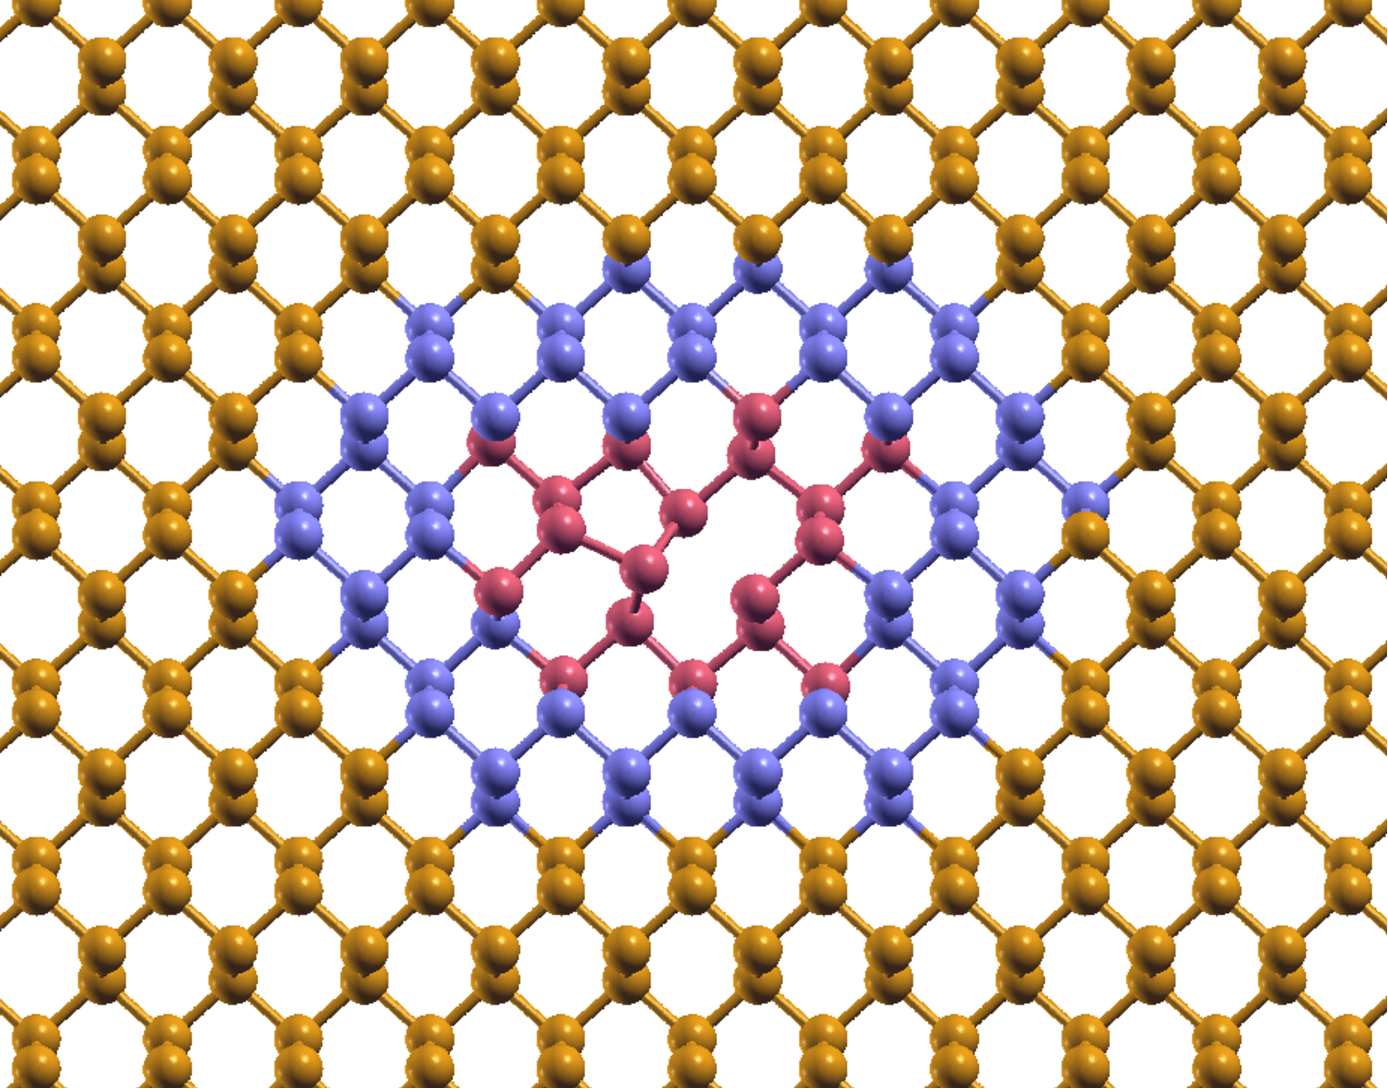
\includegraphics[width=0.3\textwidth]{67.pdf}&
  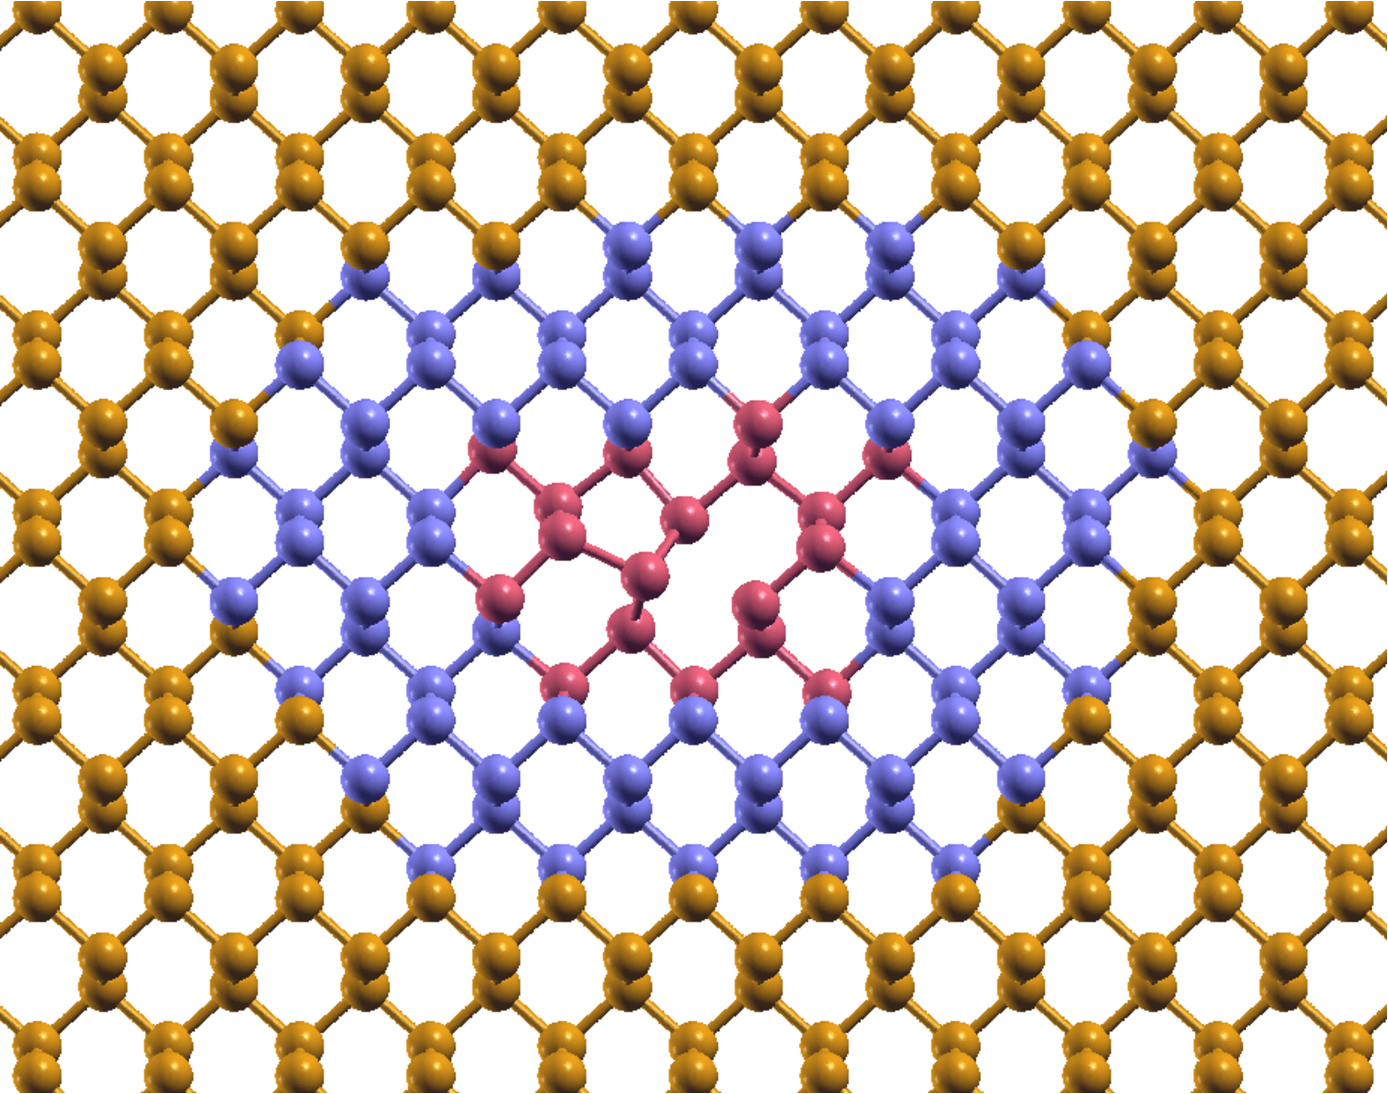
\includegraphics[width=0.3\textwidth]{88.pdf}&
  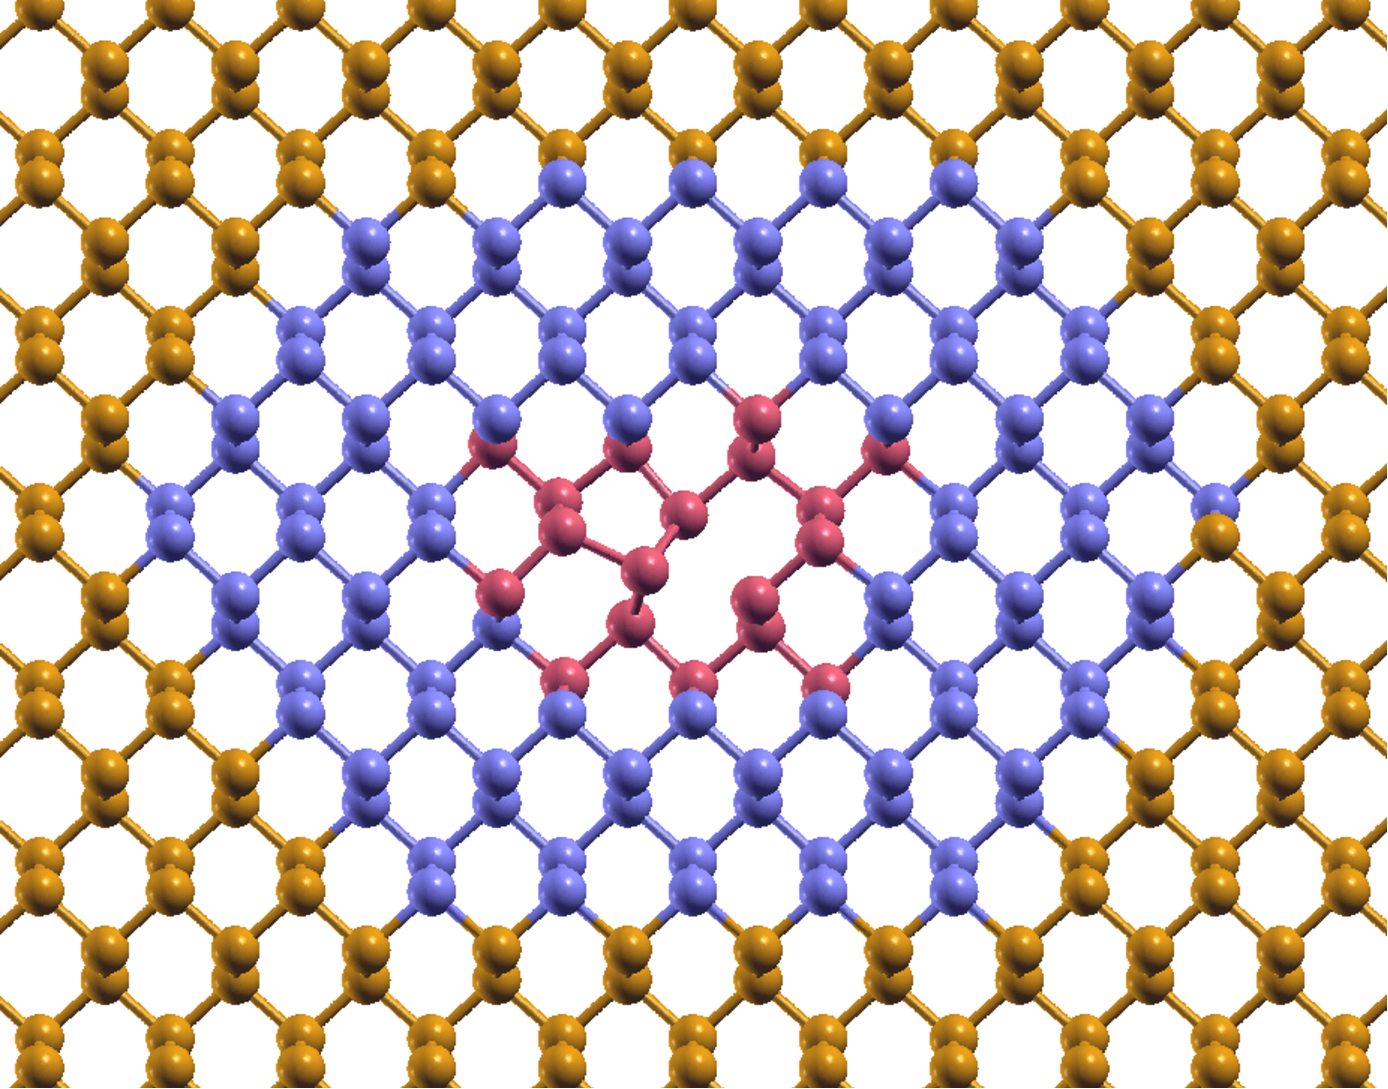
\includegraphics[width=0.3\textwidth]{114.pdf}\\
  67 atoms & 88 atoms & 114 atoms\\
  &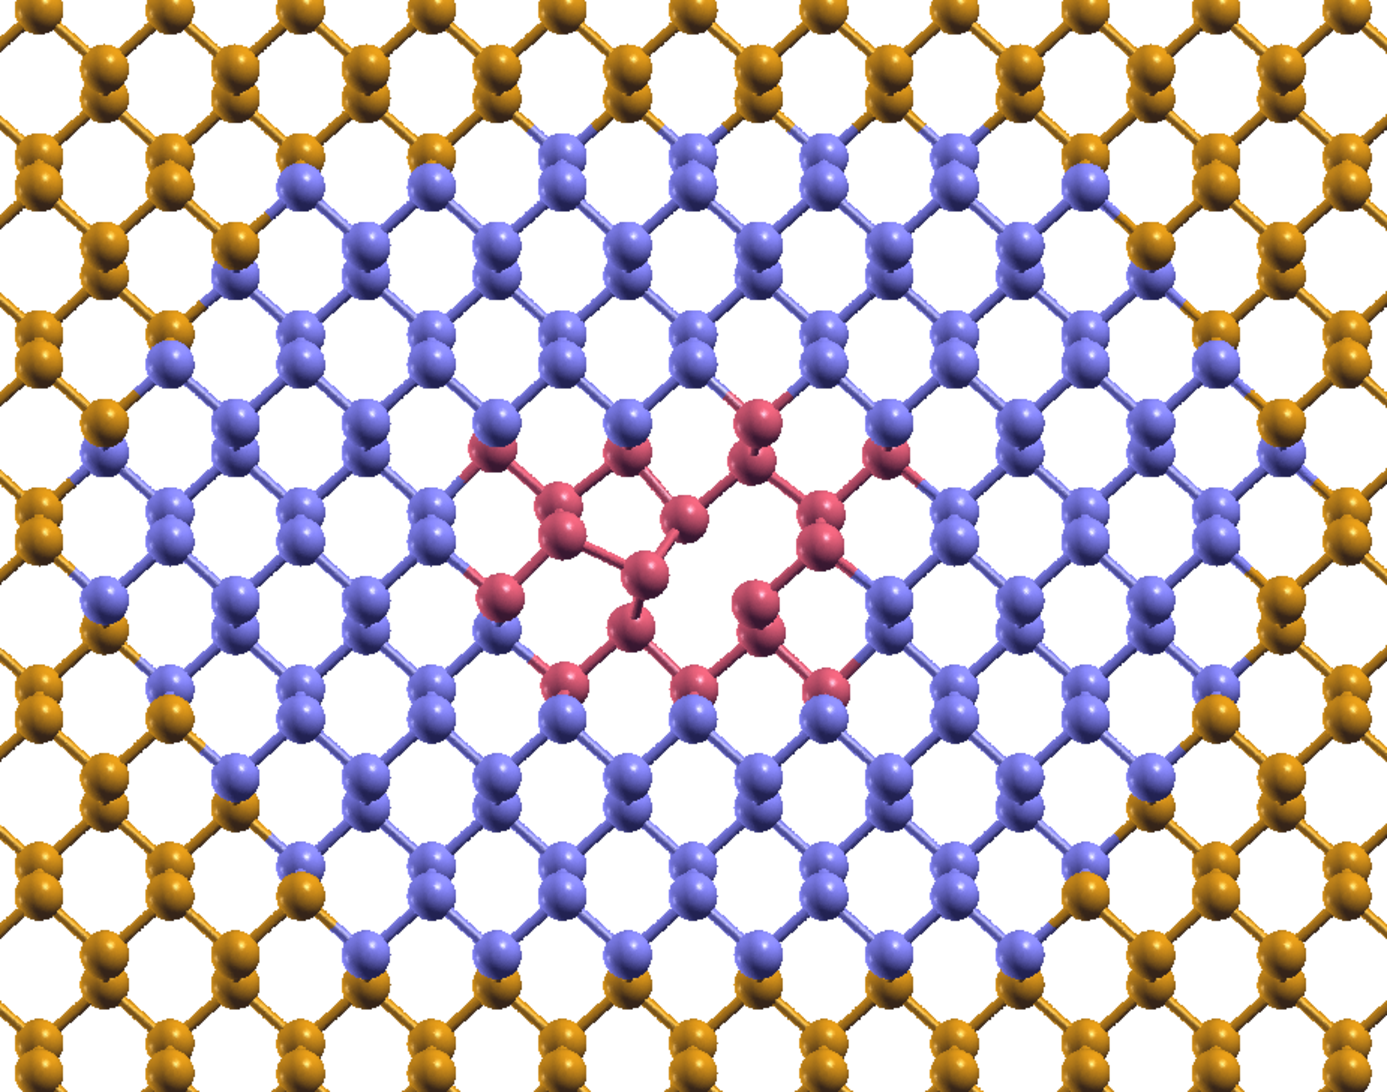
\includegraphics[width=0.3\textwidth]{141.pdf}&\\
  & 141 atoms&
\end{tabular}
\caption{Fragments used in the ADM calculations. Atoms forming the defect, i.e., those whose positions are explicitly changed, are marked in pink. These atoms, and their counterparts from the pristine structure, explicitly enter the summations over $K'$ and $K$ in Eqs.~(\ref{eq:defect_h}) and (\ref{eq:E_nuc_defect}). Fragment atoms that remain in their positions but whose electrons are relaxed within ADM are shown in pale blue. Atoms of the environment, whose electrons, represented by the resepctive WFs, are frozen and provide the embedding field, are shown in gold. The number of atoms in each fragment is indicated below the corresponding depiction.}\label{fig:frags}
\end{figure*}




Ideally, $\Delta E^{\rm ADM}$ should correspond to the thermodynamic limit, i.e., it should be converged with respect to the ADM fragment size or extrapolated to the infinite-fragment limit. The separation into HF and correlation components becomes useful here because the relatively inexpensive HF contribution, which contains most of the electrostatic and density-relaxation response to defect formation, may converge more slowly with fragment size than the more expensive correlation part. Furthermore, the correlation component itself can be partitioned into a lower-level contribution (e.g., MP2), which can be evaluated on large fragments, and a higher-level correction that is expected to converge even more rapidly.\cite{Mullan2022_JCP_Al2O3}


Technically, the ADM workflow for the present defect consists of an initial periodic calculation for pristine phosphorene, followed by orbital localization and evaluation of the electrostatic potential at the new positions of the 18 relaxed atoms. The latter enters the second term of Eq.~(\ref{eq:E_nuc_defect}). The defect is constructed by removing 19 atoms (one vacancy and 18 displaced atoms) and adding 18 atoms at their new relaxed positions. This defines the summation ranges over $K'$ and $K$ in Eqs.~(\ref{eq:defect_h}) and (\ref{eq:E_nuc_defect}). Expansion of the fragment introduces additional basis orbitals $\ket{\mu'}$ and fragment Wannier functions $N_{\rm WFs}^{\rm frag}$, and thus additional electrons to be relaxed according to Eq.~(\ref{eq:n_el}). Finally, the SCF procedure is performed for the chosen fragment using the Hamiltonian in Eq.~(\ref{eq:defect_h}) and the projected basis functions defined in Eq.~(\ref{eq:new_AO}), optionally followed by a post-Hartree-Fock treatment.



Importantly, to evaluate $\Delta E^{\rm ADM}$ consistently within ADM, both the fragment and the set of explicitly manipulated atoms entering the sums over $K'$ and $K$ in Eq.~(\ref{eq:E_nuc_defect}) must correspond one-to-one between the defect and pristine systems. This implies that $E^{\rm ADM}_{\rm pristine}$ must be computed using a fragment of the same shape as that used for $E^{\rm ADM}_{\rm defect}$. Furthermore, in the ADM calculation on the pristine structure the atoms, corresponding to the removed or displaced atoms of the defect, must be formally marked as both removed ($K$) and added ($K'$), so that they explicitly enter the effective nuclear-energy term in Eq.~(\ref{eq:E_nuc_defect}). In the present case, this corresponds to 19 atoms of the pristine system: one atom that becomes the vacancy in the defect and the 18 atoms that are displaced upon defect formation.
Due to the vacancy-type nature of the defect, the pristine ADM fragments are therefore larger by one atom than the corresponding defect fragments. 




\section{Results and Discussion}

\subsection{Defect Formation Energy}


We begin by analyzing the Hartree-Fock contribution $\Delta E^{\rm ADM}({\rm HF})$ to the defect formation energy, shown in Fig.~\ref{fig:En_form} (the numerical values are provided in the Supporting Information). 
The smallest 18-atom fragment is clearly inadequate at the HF level, which is not surprising, as for this fragment some bonding Wannier functions of the environment remain effectively anchored to the original atomic positions left behind by the displaced atoms. But even for larger fragments, the HF contribution remains far from converged, and realistic formation energies are only obtained for fragments containing 67 atoms or more. A deviation within 0.1~eV from the extrapolated value is reached only for the largest fragment considered (141 atoms). 

Despite these sizable finite-size errors for small and medium fragments, the convergence behavior is remarkably systematic. When plotted as a function of $1/N_{\rm at}^{2.8}$, the decay of $\Delta E^{\rm ADM}({\rm HF})$ becomes nearly linear over a wide range of fragment sizes, enabling a reliable extrapolation to the thermodynamic limit. Notably, this convergence is significantly faster than the $1/N_{\rm at}$ behavior expected for purely electrostatic finite-size effects of a charged defect. This observation suggests that the dominant source of the slow convergence is not long-range electrostatics, but rather the redistribution of the electronic density along the bonds induced by the structural rearrangement around the vacancy.

 




\begin{figure}
\centering
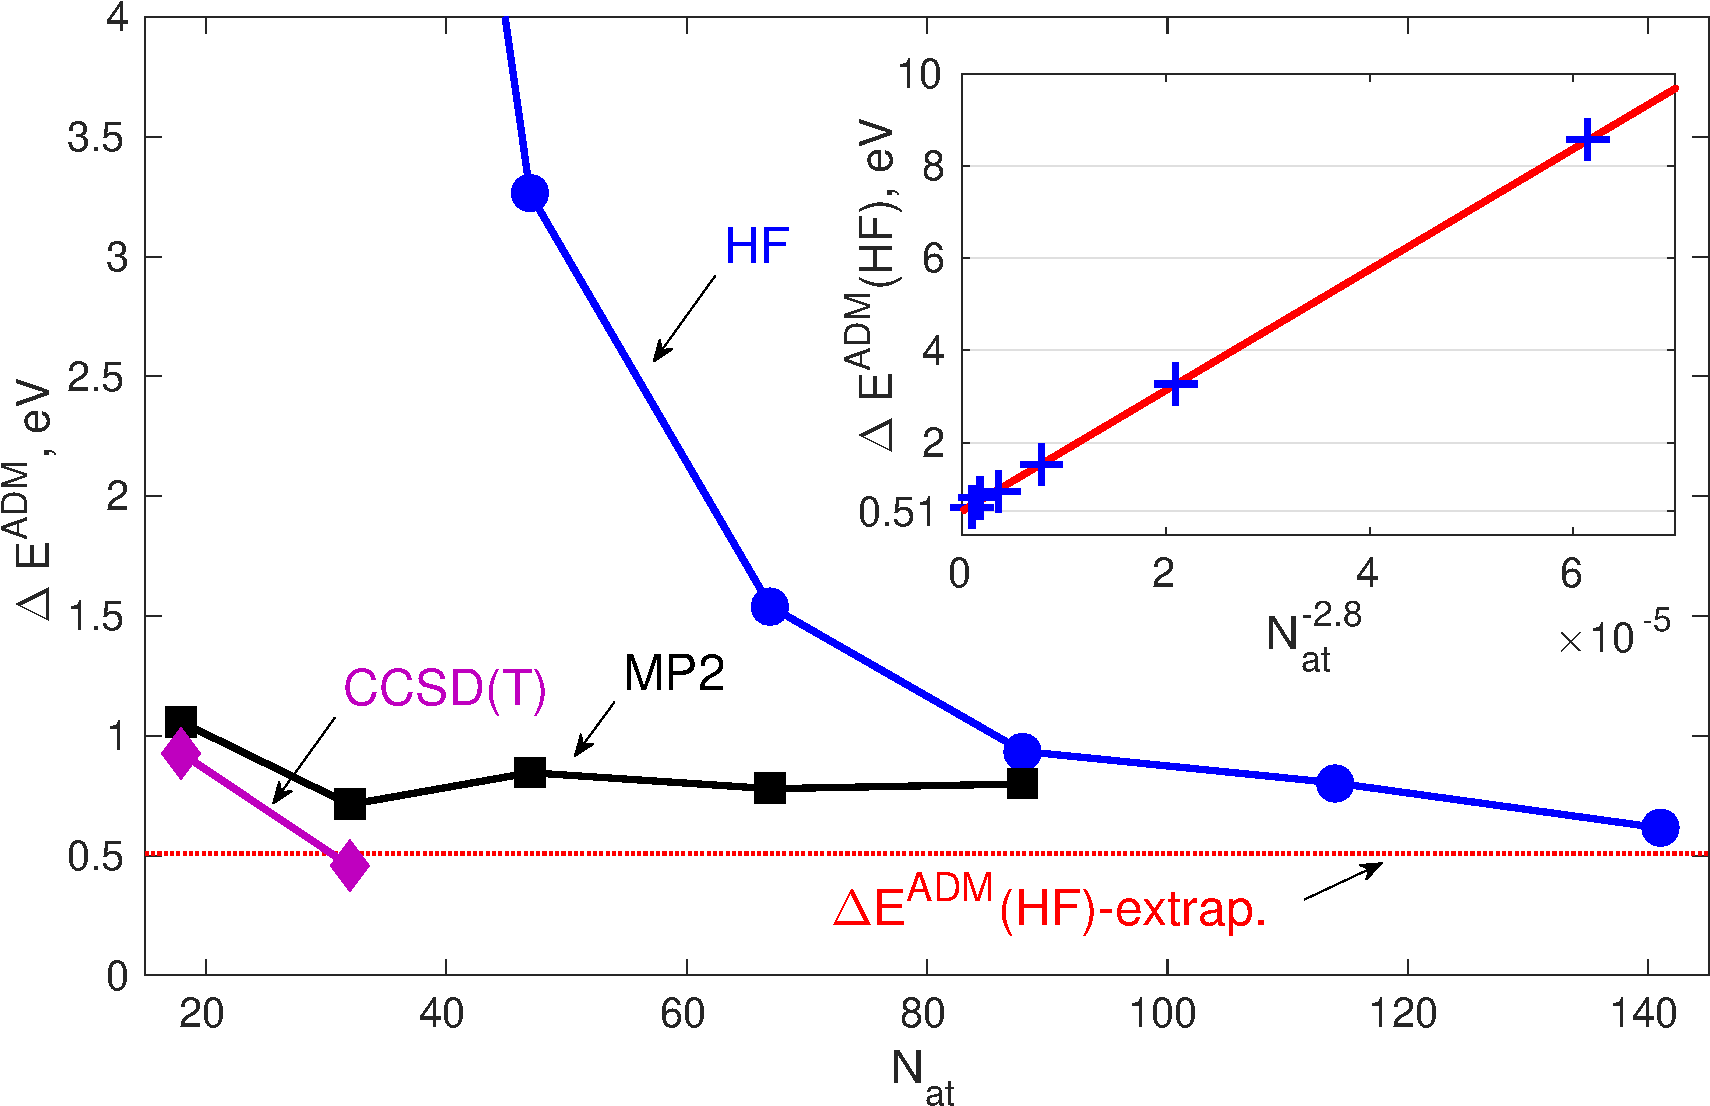
\includegraphics[width=0.45\textwidth]{E_form2.pdf}
\caption{HF and correlation components of the defect formation energy as functions of the fragment size $N_{\rm at}$. The inset shows the HF formation energies plotted as a function of $1/N_{\rm at}^{2.8}$, along with the linear fit to extrapolate to the thermodynamic limit.}
\label{fig:En_form}
\end{figure}


Although $\Delta E^{\rm ADM}({\rm HF})$ requires relatively large fragments for convergence, the computational cost of the density-fitted HF calculation remains modest, allowing the treatment of such fragment sizes. In contrast, the correlation contribution, which is computationally significantly more demanding, converges much more rapidly. Even the smallest fragment already yields meaningful values for the correlation energy, and for the second (32-atom) fragment, $\Delta E^{\rm ADM}({\rm MP2})$ is converged to within 0.1~eV.

Coupled-cluster calculations at the CCSD(T) level are too expensive to be performed beyond the 32-atom fragment. Unfortunately, for polarizable systems the convergence behavior of MP2 may differ from that of CCSD(T). In particular, long-range dispersion interactions in the latter can be effectively screened by many-body effects, which are not captured at the MP2 level.\cite{black_p_exfoliation} As a result, MP2 tends to overestimate long-range correlation contributions in such systems. This effect likely explains the more pronounced drop in $\Delta E^{\rm ADM}({\rm CCSD(T)})$ compared to MP2 when increasing the fragment size from 18 to 32 atoms. Nevertheless, since even the unscreened MP2 contribution is essentially converged at the 32-atom fragment, the CCSD(T) result can also be expected to be close to convergence.



We are now in a position to provide a CCSD(T)/POB-VTZ-rev2 estimate of the formation energy of a negatively charged monovacancy in phosphorene. The Hartree--Fock component, $\Delta E^{\rm ADM}({\rm HF})$, extrapolated to the thermodynamic limit, amounts to 0.51~eV. The correlation contribution, $\Delta E^{\rm ADM}({\rm corr})$, is evaluated as the MP2 result obtained with the 89-atom fragment (0.803~eV), combined with a CCSD(T) correction to MP2 computed with the 32-atom fragment (-0.256~eV), yielding a total correlation contribution of 0.543~eV. Finally, the relaxation correction beyond the 18-atom fragment, $\Delta E_{\rm 18\uparrow \rm relax}$, is -0.146~eV (see Sec.~\ref{sec:struct}). 
Combining these contributions gives a final estimate of the defect formation energy of $E_{\rm form} = 0.905$~eV$\approx 21$kcal/mol.
This moderate formation energy indicates that vacancy formation in phosphorene is  energetically accessible, suggesting that such defects can form under realistic conditions in appreciable concentrations, which is in agreement with experimental studies.\cite{Kiraly2017_BPvacancies,Fang2021_BPchargedVacancy}
The present value lies at the lower end of the range obtained from DFT supercell calculations for neutral vacancies (0.9 eV -- 1.7 eV).\cite{Hu2015_PhosphoreneVacancies,Naik2020_PRMaterials_PhosphoreneDefects,Rijal2021_PhosphoreneVacancy} Our benchmark, however, refers to the negatively charged defect and involves a higher-level treatment of electron correlation.


Conservative error bars associated with the remaining finite-size effects in each of the three components, $\Delta E^{\rm ADM}({\rm HF})$, $\Delta E^{\rm ADM}({\rm corr})$, and $\Delta E_{\rm 18\uparrow \rm relax}$, are expected to be below 0.1~eV. The dominant source of uncertainty is likely the basis-set incompleteness. While the POB-VTZ-rev2 basis provides a reasonable description for periodic DFT calculations, it is not guaranteed that the results are near the basis-set limit,\cite{TS_embedding} particularly for the correlation energy. In principle, ADM allows the use of different, potentially much larger molecular basis sets for the fragment calculations. However, this capability is not yet implemented in the present code, and a systematic assessment of the basis-set incompleteness error is therefore deferred to future work.


\subsection{Local correlation treatment}



With canonical high-level methods (beyond MP2), the fragment sizes required to observe a clear convergence pattern may become prohibitively large, so that convergence can often only be assessed indirectly via lower-level approaches. The underlying reason is the steep scaling of the computational cost of accurate quantum-chemical models, which can, however, be mitigated by employing local correlation schemes.\cite{Schuetz2001_LCCSD} The resulting reduced scaling of the local approach enables quantum-chemical calculations on substantially larger systems. In the present context, this allows the treatment of much larger fragments and thus a direct assessment of convergence with respect to fragment size. In this work, we employ our pilot implementation of the local distinguishable cluster method interfaced with the ADM framework.

The correlation contributions $\Delta E^{\rm ADM}({\rm corr})$ to the defect formation enegies, computed using both canonical and local methods, are compiled in Table~\ref{tab:local}. We first note that the canonical DCSD results are in good agreement with those of CCSD(T). In particular, the smaller magnitude and faster decay of $\Delta E^{\rm ADM}({\rm CCSD(T)})$ compared to MP2 are also reproduced at the DCSD level.




\begin{table}[h]
  \centering
  \caption{Correlation contribution $\Delta E^{\rm ADM}({\rm corr})$ to the defect formation energy calculated for several fragments using canonical and local correlation methods. For the local methods, the correlation energy is further partitioned into strong- and weak-pair contributions, depending on the pair types included in the pair-energy summation. Since the current implementation of LDCSD is restricted to strong pairs only, its weak-pair contribution is equal to that of LMP2.}
    \begin{tabular}{lcccccc}
    \hline\hline
    &\multicolumn{6}{c}{$N_{\rm at}$}\\
    &&18 && 32 &&47 \\
    \hline
    
    \multicolumn{7}{c}{   Canonical treatment}\\
   MP2           &~~ & 1.057 &~~ & ~0.713 &~~ & ~0.846 \\
   DCSD          & & 0.862 & & ~0.420  &&       \\
   CCSD(T)       &  & 0.927 & & ~0.457 & &       \\
    \hline
    \multicolumn{7}{c}{    Local treatement}\\
   LMP2          & & 1.074 & & ~0.713 & & ~0.838 \\
   LDCSD         & & 1.122 & & ~0.674 & & ~0.805 \\
    \hline   
   LMP2 strong   & & 0.174 & &-0.270 & & -0.254 \\
   LMP2 weak     & & 0.900 & & ~0.983 & &  ~1.092 \\
   LDCSD strong  & & 0.222  &&-0.309 & &  -0.287 \\
    \hline \hline
    \end{tabular}
    \label{tab:local}
\end{table}


The LMP2 results are in close agreement with canonical MP2, indicating that the error introduced by the local domain approximation is small. In contrast, the LDCSD results deviate significantly from canonical DCSD and instead remain close to LMP2.  To rationalize this behavior, we decompose the correlation energy into contributions from short-range (strong pairs) and long-range (weak pairs). We note that the present LDCSD implementation is restricted to strong pairs only, following the standard pair approximation employed in earlier local correlation schemes.\cite{Schuetz2001_LCCSD} As a result, the long-range correlation contribution in LDCSD is effectively described at the LMP2 level.


Analysis of the short- and long-range contributions to $\Delta E^{\rm ADM}({\rm corr})$ shows that its dominant part arises from the long-range component, i.e., from the difference in dispersive interactions between the defective and pristine systems. This observation explains why CCSD(T) and DCSD, which account for Coulomb screening of dispersion interactions, yield smaller values of $\Delta E^{\rm ADM}({\rm corr})$ compared to MP2, where dispersion is effectively unscreened. Indeed, the confinement of dispersion interactions due to screening is  known to be pronounced in polarizable systems in general and has been observed in black phosphorus or phosphorene.\cite{schuetz_usvyat_black_p}  
The dominance of the long-range contribution also supports our, albeit indirect, assessment that $\Delta E^{\rm ADM}({\rm CCSD(T)})$ converges rapidly with fragment size, as the long-range correlation is expected to decay faster at the CCSD(T) level than at the MP2 level.

Under these circumstances, if the weak-pair contribution in LDCSD remains described at the MP2 level, the accuracy of $\Delta E^{\rm ADM}({\rm LDCSD})$ cannot be expected to surpass that of MP2. This highlights the importance of a hierarchical pair approximation,\cite{Weak_pairs_schuetz_usvyat,weak_pair_werner_usvyat} in which both close and distant pairs are treated at an approximate, yet still coupled-cluster-based level. Such an approach enables an accurate and at the same time computationally affordable description of dispersion. Implementation of local correlation methods within ADM employing a proper pair treatment is currently underway.


As for the short-range correlation, which is treated at the true LDCSD level, its small but non-negligible contribution to $\Delta E^{\rm ADM}({\rm LDCSD})$ converges rapidly with fragment size, as evident from Table~\ref{tab:local}. Together with the indirect indication of the fast convergence of the long-range component, this supports the conclusion that the total high-level correlation contribution reported in Section~\ref{sec:form_en} is well converged.




\subsection{Excitation Energy}

Finally, we examine the excitation energies associated with the defect.
ADM enables a high-level quantum-chemical treatment of excited states localized on defects. A possibility for an excited-state quantum-chemical treatment is particularly significant for solid-state applications, where excited states are still mostly described at the level of the one-particle Kohn-Sham band structure.

We note that ADM is effective for states that lie within the band gap, i.e., whose excitation energies are lower than the lowest excitation energy of the host solid. Otherwise, in the absence of constraints on the excited-state wavefunction, expansion of the fragment would lead to collapse into bulk-like excited states. We illustrate the latter aspect on pristine phosphorene, subjected to a CIS excited state treatment both fully periodically and within ADM (see Fig.~\ref{fig:En_ex}). Periodic CIS, as implemented in \textsc{Cryscor}, allows one to compute the CIS optical band gap at the $\Gamma$-point. Although CIS significantly overestimates the band gap, it provides a useful reference for the relative energetic position of localized excited states.


\begin{figure}
\centering
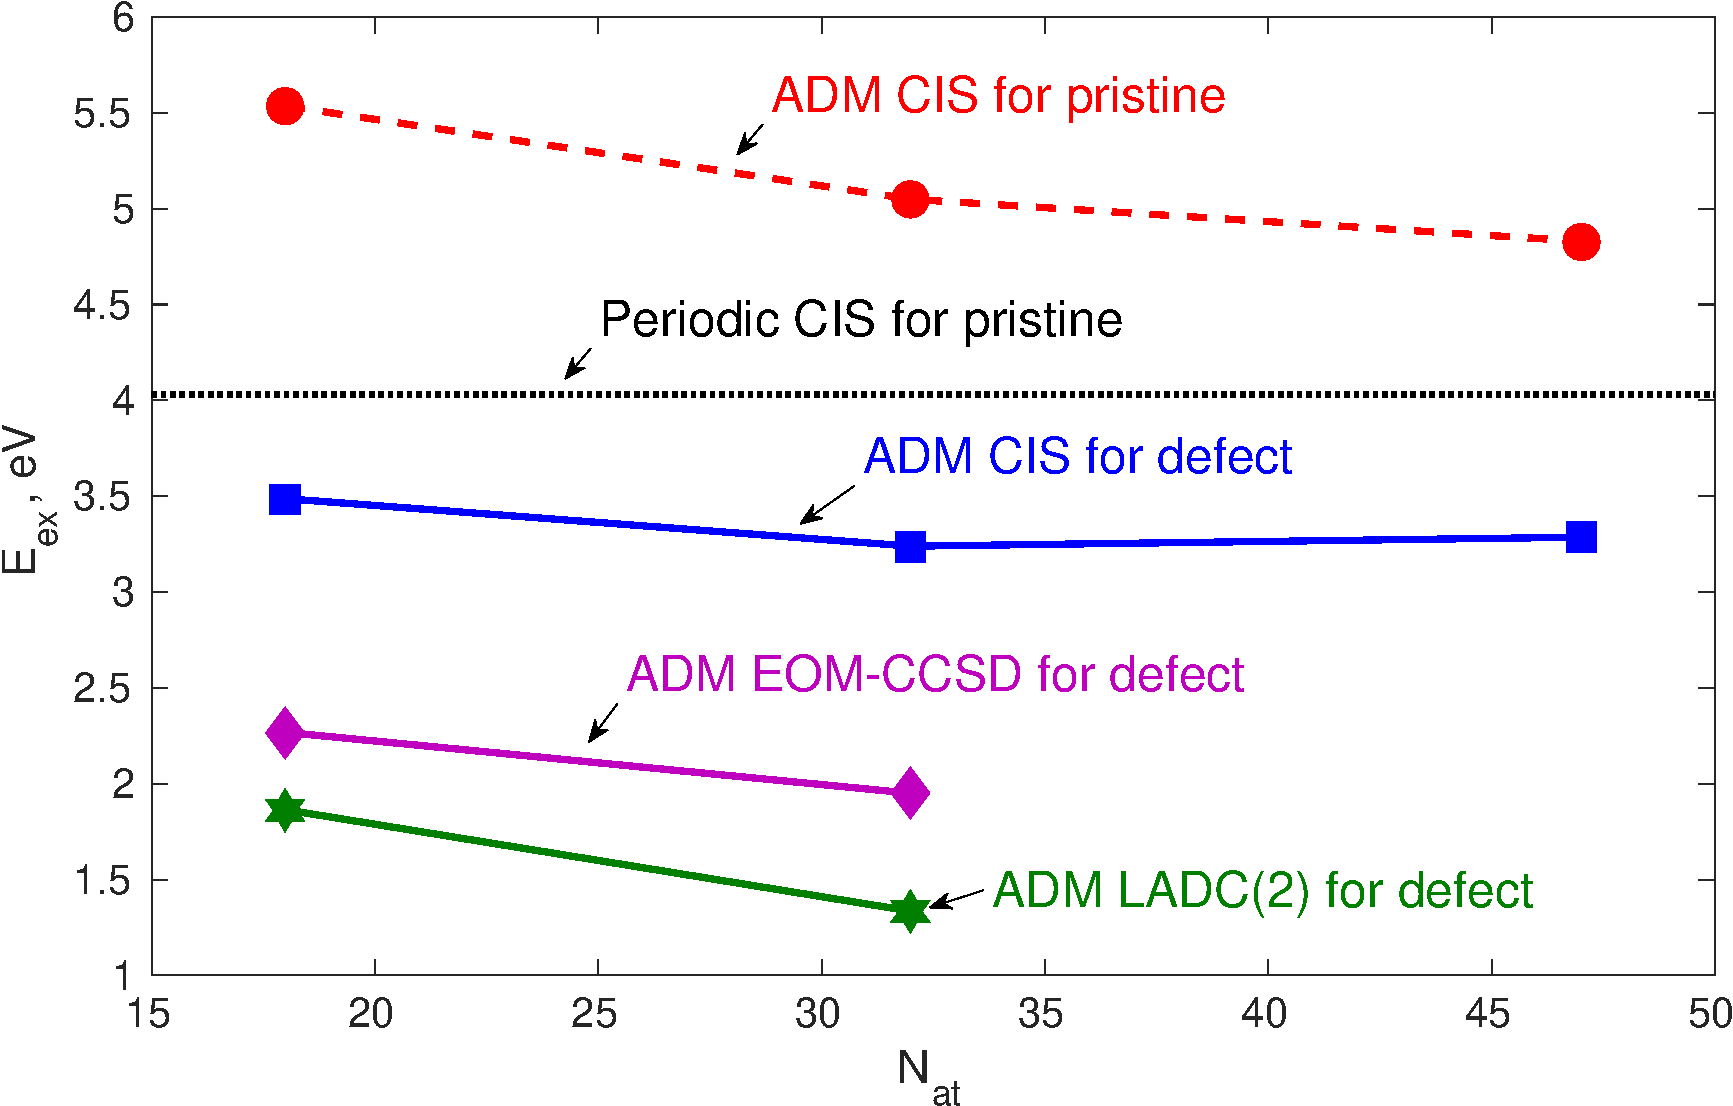
\includegraphics[width=0.45\textwidth]{E_ex2.pdf}
\caption{First excitation energy of the defect calculated using CIS, LADC(2), and EOM-CCSD methods, as well as the CIS excitation energy of pristine phosphorene computed both fully periodically and within ADM.}
\label{fig:En_ex}
\end{figure}

When pristine phosphorene is treated within ADM, the lowest excitation confined to the fragment lies well above the band gap. Upon increasing the fragment size, the excitation energy gradually decreases. In the thermodynamic limit, the ADM excited state is then expected to collapse into a delocalized bulk state and the excitation energy approach the periodic band gap.

In the case of a defect that supports localized excited states, ADM is, however, much more effective. As can be seen from Fig.~\ref{fig:En_ex}, the CIS excitation energy for the defect lies below the CIS band gap of phosphorine saturates already after a 32-atom fragment.










\section{Conclusions and Outlook}

We present a multilevel quantum embedding framework suitable for correlated studies of vacancy defects in phosphorene. The combination of periodic DFT structural optimization and HF-embedded high-level correlated treatment of defect fragments provides a path toward accurate charge-state energetics and localized electronic structure. Integration with experimental observations underscores the need for high-accuracy theoretical tools in defect engineering of 2D materials.

\bibliographystyle{unsrt}
\bibliography{citations}

\end{document}
